\chapter{Results and Discussions}
The following test case was implemented in PySPH using the method of Interface curvature described in the above sections. \\


\section{Stability of an Interface: Problem Statement}

Previous studies using the CSF formulation have reported a numerical instability at the fluid-fluid interface. \citep{rudman, Surface}. This instability leads to parasitic currents(non-zero velocities) at the interfaces. Using SPH, these currents could lead to particle disorder at the fluid-fluid interface, showing the effect of the diffusing at the interface. \\

This phenomena is studied here: A simple static case in a periodic domain spanning 0.5 units in x-direction and 1 unit in y-direction with upper half with fluid of color 1 and lower half with fluid of color 0 is simulated. The fluid densities were considered constant of 1, the surface tension coefficient to be 1 and inviscid flow is considered. The speed of sound for this simulation is set to 20 units \citep{Morris}. At t=0, a constant velocity in both directions is set so as the KE of each particle is 6 orders less than their internal energy.  The evolution of Kinetic Energy with time is recorded for different SPH parameters like smoothing length and spline. The smoothing length hdx = 1.0 and 1.5 are considered and varied smoothing length for different equations is considered where hdx = 1.0 is used all through except when calculating the surface delta function. In this way, by using a larger smoothing length for curvature calculation, more reliable estimates of curvature are obtained in the region where surface normals are non-zero.

\section{Results}

The following section shows comparision of smoothing lengths and kernels for this simulation. 

\subsection{Kernels' Comparisions}

The following plots show the comparision of the solutions for different kernels for various smoothing lengths: h1 = 1.0, h2 = 1.5 and variedh case where different smoothing length is used for different parts of the simulation.

\begin{figure}[H]
\centering
\begin{subfigure}[b]{0.45\textwidth}
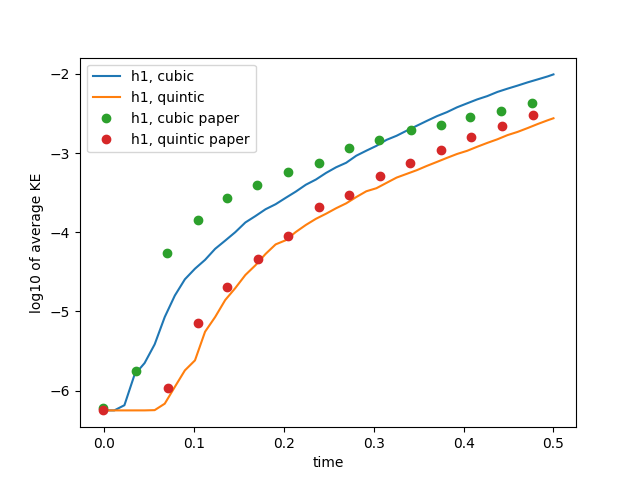
\includegraphics[width=\linewidth]{./case10.png}
\caption{h=h1=1.0}
\end{subfigure}
\begin{subfigure}[b]{0.45\textwidth}
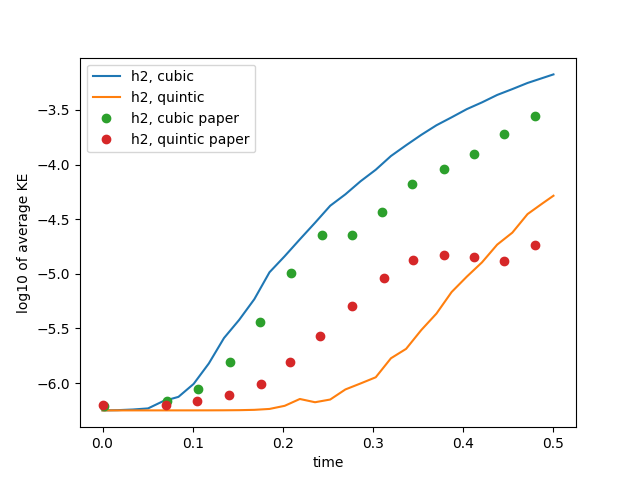
\includegraphics[width=\linewidth]{./case11.png}
\caption{h=h2=1.5}
\end{subfigure}

\begin{subfigure}[b]{0.5\textwidth}
\centering
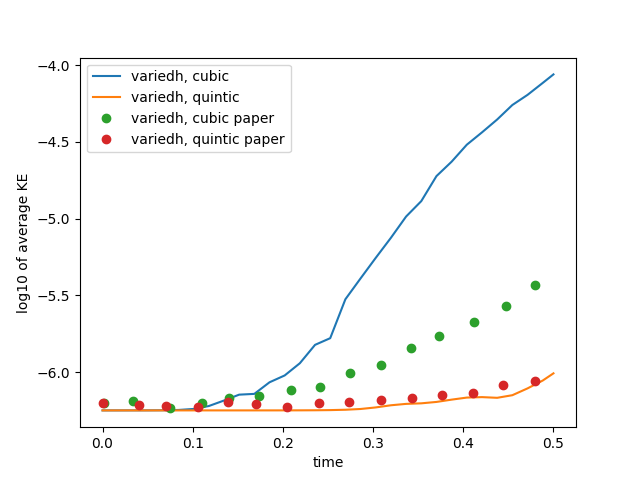
\includegraphics[width=\linewidth]{./case12.png}
\caption{Varied smoothing length}
\end{subfigure}
\caption{Variation of KE for different smoothing lengths}
\end{figure}

In all the cases it can be clearly seen that the Quintic spline has better stability with lower diffusion and KE than the cubic spline. The variations in results when compared to \citep{Morris} as the initializations used are not exactly random(as it was not explained in the paper how the initializations were done),
we used a constant velocity in both the dimensions and the magnitude was used so as to match, the initial KE. 

\subsection{Smoothing Lengths' Comparisions}

The following plots show the comparisions of the solutions for different smoothing lengths for various kernels: Cubic spline and Quintic Spline

\begin{figure}[H]
\centering
\begin{subfigure}[b]{0.45\textwidth}
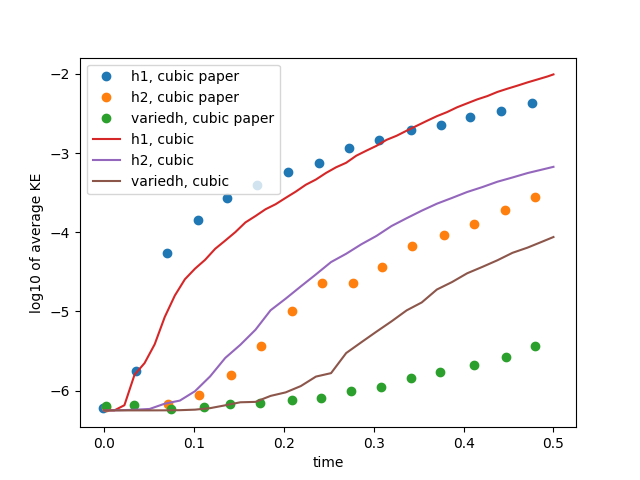
\includegraphics[width=\linewidth]{./case13.png}
\caption{Cubic Spline}
\end{subfigure}
\begin{subfigure}[b]{0.45\textwidth}
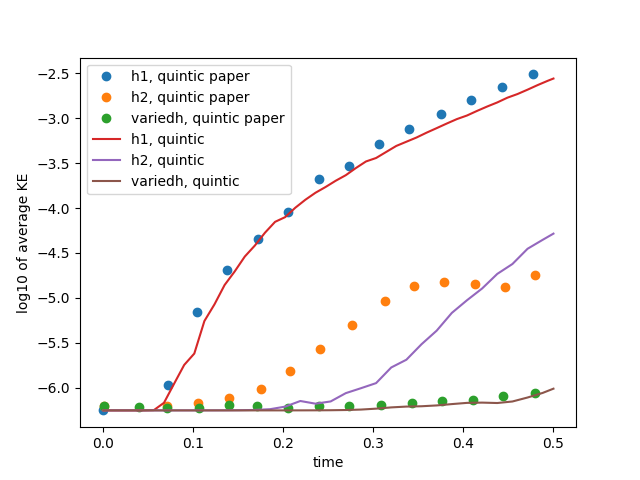
\includegraphics[width=\linewidth]{./case14.png}
\caption{Quintic Spline}
\end{subfigure}
\caption{Variation of KE for different Kernels}
\end{figure}

In all the cases, it can be noted that the varied smoothing lengths when used give the best solution preventing diffusion, then h2=1.5 and h1=1.0 has the worst simulation. 

\section{Discussions}

It can be seen from the plot that the variableh case has better stability of the interface preventing much diffusion of the particles into each other.\\

It is seen that, for the same parameters, the quintic spline is more stable than the cubic spline.\\

Also, the increased smoothing length caused to a considerable amount of stability in the interface. The best stability properties are however exhibited when the smoothing length for curvature is higher than that of delta function calculation.

